\documentclass[11pt]{article}
\usepackage[margin=1in]{geometry}
\usepackage{volfit_preamble}
\graphicspath{{figures/}}

\title{\textbf{The LQD Model, from Distribution to Smile}\\[2pt]
\large An alternative lecture on log-quantile-density parametrization\\[2pt]
\normalsize Vol-Fitter Technical Notes, No.~01}
\author{Vol-Fitter}
\date{\today}

\begin{document}
\maketitle

% Auto-generated by Docs/notes/figures/gen_lqd.py — do not edit.
\newcommand{\lqdoptpts}{2001}
\newcommand{\lqdbarriercenter}{0.90}
\newcommand{\lqdbarrierscale}{50.0}
\newcommand{\lqdsviAL}{0.214458}
\newcommand{\lqdsviAR}{0.069023}
\newcommand{\lqdsvimu}{0.020613}
\newcommand{\lqdsvibetaL}{0.097073}
\newcommand{\lqdsvibetaR}{0.035757}
\newcommand{\lqdsvimaxerr}{0.23}
\newcommand{\lqdsvisigma}{20.62}
\newcommand{\lqdsviskew}{-0.3538}
\newcommand{\lqdsvicurv}{1.6474}
\newcommand{\lqdsvimart}{0.00e+00}
\newcommand{\lqdsvinfev}{7}
\newcommand{\lqdsvicoefftable}{\begin{tabular}{lr} \toprule Parameter & Value\\ \midrule $L$ & -1.87479110\\ $R$ & -3.08957252\\ $a_{2}$ & +0.38076853\\ $a_{3}$ & -0.04700855\\ $a_{4}$ & -0.00719617\\ $a_{5}$ & +0.00645578\\ $a_{6}$ & +0.00213226\\ \bottomrule \end{tabular}}
\newcommand{\lqddhmaxerr}{13.19}
\newcommand{\lqddhAL}{0.015341}
\newcommand{\lqddhAR}{0.014979}
\newcommand{\lqdtimingtable}{\begin{tabular}{rrrrrr} \toprule $N$ & $P$ & analytic (ms) & FD (ms) & speed-up & $|\Delta\mathrm{cost}|$\\ \midrule 6 & 7 & 15.3 & 25.0 & 1.64$\times$ & 5.6e-20\\ 8 & 9 & 20.9 & 29.2 & 1.40$\times$ & 1.4e-19\\ 10 & 11 & 26.6 & 41.7 & 1.57$\times$ & 8.9e-20\\ 12 & 13 & 27.3 & 47.0 & 1.72$\times$ & 2.0e-20\\ \bottomrule \end{tabular}}

\IfFileExists{figures/lqd_lecture_tables.tex}{
  % Auto-generated by Docs/notes/figures/gen_lqd_lecture.py -- do not edit.
\newcommand{\lqdlecturescale}{0.078}
\newcommand{\lqdlectureexpiry}{0.5}
\newcommand{\lqdlecturemu}{-0.010028}
\newcommand{\lqdlectureatm}{19.20}
\newcommand{\lqdlectureuatm}{0.5321}
\newcommand{\lqdlectureAL}{0.078}
\newcommand{\lqdlectureAR}{0.078}
\newcommand{\lqdlecturebetaL}{0.0375}
\newcommand{\lqdlecturebetaR}{0.0406}
\newcommand{\lqdlecturemart}{0.00e+00}

}{
  \newcommand{\lqdlecturescale}{0.078}
  \newcommand{\lqdlectureexpiry}{0.5}
  \newcommand{\lqdlecturemu}{-0.010028}
  \newcommand{\lqdlectureatm}{19.20}
  \newcommand{\lqdlectureuatm}{0.5321}
  \newcommand{\lqdlectureAL}{0.078}
  \newcommand{\lqdlectureAR}{0.078}
  \newcommand{\lqdlecturebetaL}{0.0375}
  \newcommand{\lqdlecturebetaR}{0.0406}
  \newcommand{\lqdlecturemart}{0.00e+00}
}

\begin{abstract}
A smile is a probability distribution wearing option-market clothes.  The LQD
model takes that sentence literally: instead of drawing implied volatility and
then asking whether the resulting curve hides a negative density, it draws an
increasing quantile function and prices the smile from the resulting law.  For
the log-forward return $X$, the model writes the logarithm of the quantile
density as a universal two-sided tail skeleton plus a short Legendre expansion.
Positivity is then automatic, a single additive shift enforces the forward
martingale, and the endpoint scales identify both the last finite moments and
the Lee wing slopes.  This lecture develops the construction from a concrete
logistic slice, proves the one-expiry no-butterfly result, derives pricing,
tails, exact ATM level/skew/curvature identities, calibration, the analytic
price Jacobian, and soft cross-expiry control.  It then follows the production
calibrator through two deterministic approximation cases: a seven-parameter
fit to an SPX-like SVI target with maximum quote-grid error
\lqdsvimaxerr\ volatility basis points, and a thirteen-parameter fit that
qualitatively recovers a two-humped event density.  The emphasis throughout is
on the few facts that carry the model; numerical plumbing and control tables
are kept out of their way.
\end{abstract}

\tableofcontents
\newpage

%======================================================================
\section{The desk problem: do not manufacture negative probability}
\label{sec:desk}

Imagine fitting a quiet expiry with seven liquid strikes.  The quoted vols are
unremarkable; the interpolated smile looks smooth; the residuals are tiny.
Then someone asks for a tight butterfly between two quote nodes.  The model
returns a negative price.  Nothing dramatic happened on the screen.  The curve
was simply smooth in the wrong coordinate, and its second strike derivative
changed sign between observations.

That failure is easy to explain after the fact.  A call curve must be decreasing
and convex in strike, because its second strike derivative is a risk-neutral
density.  A generic interpolant in implied volatility does not know this.
There are perfectly good direct-price and constrained-SVI approaches, but they
must encode or police the same global condition.  LQD makes a different trade:
it starts from a probability law, where non-negative mass is local and cheap,
then integrates to option prices.

\begin{invariant}
\begin{enumerate}[leftmargin=1.6em]
\item Every feasible one-expiry parameter vector defines a continuous,
non-negative probability density and therefore a butterfly-free call slice.
\item The normalized underlying has mean one.  This requires one scalar shift
and, for the LQD tail family, the hard condition $A_R<1$.
\item Tail behaviour is part of the distribution, not an extrapolation patch:
the endpoint scales determine the critical moments and Lee slopes.
\item The trader handles --- ATM volatility, log-strike skew and curvature ---
are analytic functionals of the constructed slice, not finite differences of
an IV grid.
\end{enumerate}
\end{invariant}

\subsection{Normalize first, so carry does not clutter the mathematics}

Fix an expiry date $T$.  Let $F_T$ and $D_T$ be its forward and discount factor,
and define
\begin{equation}
Y=\frac{S_T}{F_T},\qquad X=\log Y,\qquad
k=\log\frac{K}{F_T}.
\label{eq:variables}
\end{equation}
Under deterministic carry and the $T$-forward measure,
\begin{equation}
\E[Y]=\E[e^X]=1.
\label{eq:martingale}
\end{equation}
The normalized undiscounted call is
\begin{equation}
C(k)=\frac{C^\$(F_Te^k,T)}{D_TF_T}
     =\E\!\left[(e^X-e^k)^+\right].
\label{eq:call_expectation}
\end{equation}
All slice formulas below live in these units.  Dollars return only at the outer
API boundary.

\paragraph{The two clocks.}
$T$ labels an expiry date; $\tau$ denotes the year fraction used for variance
annualization.  In production, $\tau$ is the active variance time supplied as
\texttt{prepared.tau}: it equals calendar time when the event clock of Note~11
is inactive, and otherwise includes scheduled-event dilation.  Thus
$w=\sigma^2\tau$ and Black vega is $\phin(d_+)\sqrt{\tau}$.  Keeping $\tau$
visible avoids the common mistake of mixing carry time with variance time.

\subsection{The model in one equation}

Let $Q(u)$ be the quantile of $X$ at percentile $u\in(0,1)$ and
$q(u)=Q'(u)$ its quantile density.  LQD stands for
\emph{log quantile density}: it models $\ell(u)=\log q(u)$ as
\begin{equation}
\boxed{\;
\ell(u)=-\log u-\log(1-u)+(1-u)L+uR
       +\sum_{n=2}^{N}a_nP_n(1-2u)\; .}
\label{eq:lqd}
\end{equation}
Here $P_n$ is the $n$th Legendre polynomial.  The shipped order $N=6$ has the
seven coefficients $(L,R,a_2,\ldots,a_6)$; the API accepts
$4\le N\le16$.

There are only three ideas in \eqref{eq:lqd}.
\begin{enumerate}[leftmargin=1.6em]
\item Taking a logarithm makes $q=e^\ell$ positive for every finite coefficient
vector.  Hence $Q$ is increasing and cannot fold probability mass over itself.
\item The terms $-\log u-\log(1-u)$ impose controllable exponential tails on
$X$, hence power tails on $Y=e^X$ and linear total-variance wings.
\item A short orthogonal-polynomial expansion bends the distribution between
the endpoints.
\end{enumerate}

One warning is worth placing beside the definition.  $L$ and $R$ are convenient
low-order endpoint \emph{coordinates}; once $a_n\ne0$, they are not the log tail
scales.  Every Legendre mode reaches both endpoints.  The actual tail handles
$A_L,A_R$ will appear in \cref{sec:tails}.

The full pipeline is
\[
(L,R,a_2,\ldots,a_N)
\longrightarrow q
\longrightarrow Q
\longrightarrow \text{mean-one shift}
\longrightarrow C(k)
\longrightarrow \sigma_{\rm imp}(k).
\]
In production, structural density positivity is still visible in one line:
\begin{lstlisting}[caption={The non-negative return density, distilled from
\texttt{backend/volfit/models/lqd/quadrature.py}.},
label={lst:density_crux}]
def density_at_quantile(u, g):
    # q(u) = exp(g(u)) / (u * (1-u))
    return u * (1-u) * np.exp(-g)  # f_X(Q(u)) = 1/q(u) >= 0
\end{lstlisting}

%======================================================================
\section{A probability ruler instead of a volatility curve}
\label{sec:ruler}

The cleanest way to read a quantile model is to start with a uniform random
variable.  Let $U\sim{\rm Uniform}(0,1)$ and set
\begin{equation}
X=Q(U).
\label{eq:pushforward}
\end{equation}
If $Q$ is strictly increasing, this construction assigns exactly $u$ units of
probability below $Q(u)$.  Where a density exists, differentiating
$F_X(Q(u))=u$ gives
\begin{equation}
f_X(Q(u))Q'(u)=1,\qquad
f_X(Q(u))=\frac{1}{q(u)}.
\label{eq:density_inverse}
\end{equation}
A large $q$ means that a wide interval of returns is needed to accommodate a
small interval of probability: the ordinary density is thin there.  A small
$q$ means probability percentiles are packed together: the ordinary density
is high.  Quantile density and ordinary density are reciprocal views of the
same ruler.

\subsection{Why positivity of the ruler kills butterflies}

Let $y=e^k$ be normalized strike and
$\widetilde C(y)=\E[(Y-y)^+]$.  When $Y$ has a density,
\begin{equation}
\frac{\partial \widetilde C}{\partial y}=-(1-F_Y(y)),
\qquad
\frac{\partial^2\widetilde C}{\partial y^2}=f_Y(y)\ge0.
\label{eq:breeden_litzenberger}
\end{equation}
This is the Breeden--Litzenberger identity.  It is useful intuition, but the
no-butterfly proof is even shorter.

\begin{proposition}[Structural butterfly freedom]
\label{prop:butterfly}
Suppose $\overline Q$ is strictly increasing and
$M=\int_0^1e^{\overline Q(u)}\dd u$ is finite.  Define
$Q=\overline Q-\log M$.  Then \eqref{eq:call_expectation} is the call curve of
a positive mean-one random variable.  It is decreasing and convex in normalized
strike, satisfies put--call parity, and is free of butterfly arbitrage.
\end{proposition}

\begin{proof}
With $U$ uniform, $Y=e^{Q(U)}$ is positive and
$\E[Y]=e^{-\log M}M=1$.  A call is the expectation of the convex payoff
$(Y-y)^+$.  Its strike monotonicity and convexity follow either pointwise from
the payoff or from \eqref{eq:breeden_litzenberger}; parity follows by subtracting
the corresponding put payoff.  No density-positivity constraint is left for
the optimizer.
\end{proof}

The proposition is deliberately modest.  LQD spans a finite-dimensional
\emph{subset} of continuous densities; it does not claim to represent every
density.  And the statement is for one expiry.  Cross-expiry calendar
arbitrage is a separate question (\cref{sec:calendar}).  The scalar
normalization translates the log-return law and rescales $Y$, but
$Q'=\overline Q'$: quantile-density shape and tail slopes are unchanged.

\subsection{Pricing directly on percentiles}

Let $u_k$ solve $Q(u_k)=k$.  Only percentiles above $u_k$ finish in the money,
so
\begin{align}
C(k)
  &=\int_{u_k}^{1}\left(e^{Q(u)}-e^k\right)\dd u,
\label{eq:call_u}\\
P(k)
  &=\int_{0}^{u_k}\left(e^k-e^{Q(u)}\right)\dd u.
\end{align}
Subtracting the two integrals and using $\int_0^1e^{Q(u)}\dd u=1$ gives
$C(k)-P(k)=1-e^k$.

%======================================================================
\section{The logistic slice: the whole machine in one toy}
\label{sec:logistic}

Before adding a single polynomial, set
\begin{equation}
a_n=0,\qquad L=R=\log s,\qquad 0<s<1.
\label{eq:logistic_setup}
\end{equation}
Then
\[
q(u)=\frac{s}{u(1-u)},\qquad
Q(u)=\mu+s\log\frac{u}{1-u}.
\]
So $X$ is logistic with scale $s$, shifted by $\mu$.  The martingale integral
is a beta integral:
\begin{equation}
\E[e^X]
=e^\mu\int_0^1u^s(1-u)^{-s}\dd u
=e^\mu B(1+s,1-s)
=e^\mu\frac{\pi s}{\sin(\pi s)}.
\end{equation}
Consequently
\begin{equation}
\mu=-\log\frac{\pi s}{\sin(\pi s)},\qquad s<1,
\label{eq:logistic_mu}
\end{equation}
and $\Var(X)=\pi^2s^2/3$.  The same inequality $s<1$ that makes the beta
integral finite will later become the general right-tail condition $A_R<1$.

\begin{figure}[H]
\centering
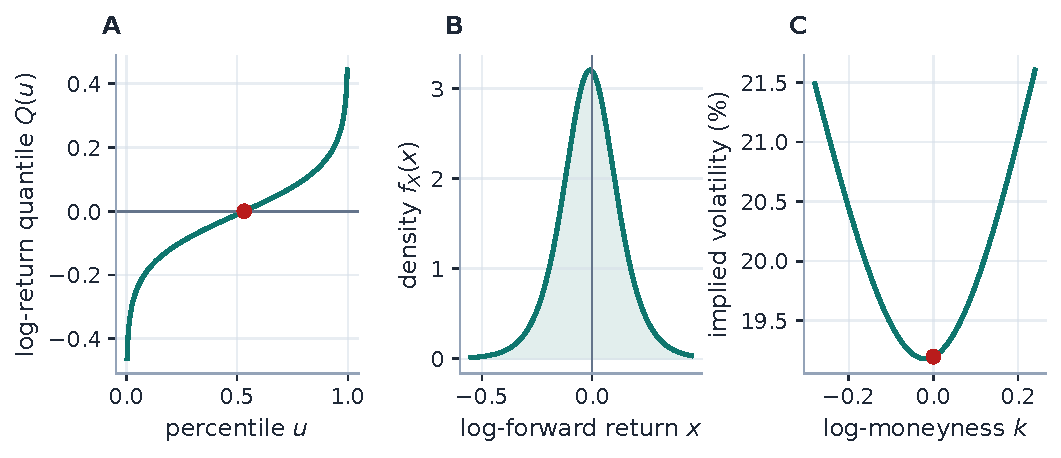
\includegraphics[width=\textwidth]{fig_lqd_logistic_lecture.pdf}
\caption{One law, three market languages.  A logistic LQD slice with
$s=\lqdlecturescale$ becomes an increasing log-return quantile (A), a
non-negative density (B), and a half-year implied-volatility smile (C).  The
red dot follows the forward strike: martingale normalization places
$Q(u)=0$ at $u=\lqdlectureuatm$, not at the median, so a symmetric
log-return shape does not imply a perfectly symmetric Black smile.}
\label{fig:logistic}
\end{figure}

The plotted half-year slice has $\mu=\lqdlecturemu$, ATM volatility
\lqdlectureatm\%, and a martingale self-check of
$\E[e^X]-1=\lqdlecturemart$.  Its two endpoint scales both equal
\lqdlecturescale, but the left and right Lee slopes differ:
\lqdlecturebetaL\ and \lqdlecturebetaR.  The difference comes from the
martingale moment on the right: a finite forward consumes one power of $Y$.

\begin{example}[title={Example: why the cold start is close, but not exact}]
Production initializes $s$ from the heuristic variance match
$w_{\rm ATM}\approx\Var(X)=\pi^2s^2/3$.  This is intentionally cheap; ATM
implied variance is not log-return variance.  In fact, as $s\downarrow0$,
\[
C(0)\sim s\log2,\qquad
\Black(0,w)\sim\sqrt{\frac{w}{2\pi}},
\qquad
w_{\rm ATM}\sim2\pi(\log2)^2s^2.
\]
The variance-match coefficient is about $8\%$ larger.  The initializer only
needs to land in the right basin; the nonlinear fit supplies the correction.
\end{example}

The logistic law is therefore more than a classroom special case.  It is a
complete admissible slice, an analytic check on normalization and tails, and
the actual cold-start family used by \texttt{logistic\_init}.

%======================================================================
\section{Why the LQD formula has exactly this shape}
\label{sec:shape}

\subsection{The logit coordinate removes both endpoint singularities}

Write the smooth part of \eqref{eq:lqd} as
\begin{equation}
g(u)=(1-u)L+uR+\sum_{n=2}^{N}a_nP_n(1-2u).
\label{eq:g}
\end{equation}
The divergence of $q=e^g/[u(1-u)]$ is real: it creates the return tails.
The logit coordinate absorbs that divergence into a finite tail slope.  Set
\begin{equation}
z=\log\frac{u}{1-u},\qquad
u=\Lambda(z)=\frac{1}{1+e^{-z}},\qquad
\frac{\dd u}{\dd z}=u(1-u).
\label{eq:logit}
\end{equation}
The two endpoint factors cancel:
\begin{equation}
\frac{\dd Q}{\dd z}
=\frac{\dd Q}{\dd u}\frac{\dd u}{\dd z}
=\frac{e^{g(u)}}{u(1-u)}u(1-u)
=e^{g(\Lambda(z))}>0.
\label{eq:qz}
\end{equation}
This is the operative equation in code.  The open percentile interval
$(0,1)$ has become the real line, and the quantile is the integral of a smooth
positive function:
\begin{equation}
\overline Q(z)=\int_0^z e^{g(\Lambda(r))}\dd r.
\label{eq:qbar}
\end{equation}

\begin{heuristic}
Think of $z$ as a probability ruler with evenly spaced tail marks.  The function
$e^g$ is the local exchange rate between that ruler and log return.  Large
$e^g$ stretches return space and thins the density; small $e^g$ compresses
return space and piles probability up.  Positivity says the ruler may stretch
or compress, but it may never run backwards.
\end{heuristic}

\subsection{Why Legendre polynomials, and why start at degree two?}

With $x=1-2u$, Legendre polynomials obey
\begin{equation}
\int_0^1P_m(1-2u)P_n(1-2u)\dd u
=\frac{\1_{m=n}}{2n+1}.
\label{eq:legendre_orthogonality}
\end{equation}
They provide a numerically well-scaled global basis on the percentile interval.
The constant and linear degrees are already carried by
\begin{equation}
(1-u)L+uR
=\frac{L+R}{2}+\frac{L-R}{2}(1-2u),
\end{equation}
so the explicit sum begins at $n=2$.  At $N=6$ the model spans the same
polynomial space as $P_0,\ldots,P_6$, while retaining two readable baseline
endpoint coordinates.

The word \emph{body mode} can mislead.  Legendre polynomials are global:
$P_n(1)=1$ and $P_n(-1)=(-1)^n$.  A coefficient that sculpts the centre also
moves one or both endpoint scales.  Orthogonality improves conditioning; it
does not localize the parameters.  Production evaluates the basis by the
three-term recursion
\begin{equation}
(n+1)P_{n+1}(x)=(2n+1)xP_n(x)-nP_{n-1}(x),
\qquad P_0=1,\quad P_1=x.
\label{eq:legendre_recursion}
\end{equation}

%======================================================================
\section{The wings know their moments}
\label{sec:tails}

\subsection{Endpoint scales are the genuine tail handles}

Because $g$ is continuous at both endpoints,
\begin{align}
A_L:=e^{g(0)}
  &=\exp\!\left(L+\sum_{n=2}^{N}a_n\right), \label{eq:AL}\\
A_R:=e^{g(1)}
  &=\exp\!\left(R+\sum_{n=2}^{N}(-1)^na_n\right).
\label{eq:AR}
\end{align}
Integrating $q(u)\sim A_L/u$ on the left and
$q(u)\sim A_R/(1-u)$ on the right gives finite constants $B_L,B_R$ such that
\begin{equation}
Q(u)=B_L+A_L\log u+o(1)\quad(u\downarrow0),
\qquad
Q(u)=B_R-A_R\log(1-u)+o(1)\quad(u\uparrow1).
\label{eq:quantile_tails}
\end{equation}
Thus $X$ has exponential tails.  Equivalently, $Y=e^X$ has power tails.  This
is a modelling assumption, not a mere numerical convenience.

\subsection{One integral gives the moment strip and the hard wall}

For any real $r$,
\[
\E[e^{rX}]=\int_0^1e^{rQ(u)}\dd u.
\]
Using \eqref{eq:quantile_tails}, the left integrand behaves like $u^{rA_L}$
and the right like $(1-u)^{-rA_R}$.  Therefore
\begin{equation}
\E[e^{rX}]<\infty
\quad\Longleftrightarrow\quad
-\frac{1}{A_L}<r<\frac{1}{A_R}.
\label{eq:moment_strip}
\end{equation}
Setting $r=1$ proves the load-bearing admissibility condition
\begin{equation}
A_R<1.
\label{eq:finite_forward}
\end{equation}
For finite coefficients this condition is necessary and sufficient for the
forward moment.  The left tail needs no analogous restriction because
$A_L>0$ already makes $r=1$ integrable there.

\begin{caution}
$A_R=1$ is not a regularization preference.  At that wall the normalized
underlying has infinite mean, so no finite forward exists.  Production keeps a
$10^{-6}$ buffer, rejects $A_R\ge1-10^{-6}$, and adds a soft barrier centred at
\lqdbarriercenter\ to turn the optimizer back before rejection.  The barrier is
smooth inside the feasible region; the switch to the infeasible penalty branch
is not an algebraic continuation through the wall.
\end{caution}

\subsection{From critical moments to Lee slopes}

For $Y=e^X$, define the last finite extra right moment and inverse left moment
\begin{equation}
p_+=\sup\{p\ge0:\E[Y^{1+p}]<\infty\}
    =\frac{1}{A_R}-1,
\qquad
p_-=\sup\{p\ge0:\E[Y^{-p}]<\infty\}
    =\frac{1}{A_L}.
\label{eq:critical_moments}
\end{equation}
Lee's moment map is
\begin{equation}
\psi(p)=2-4\left(\sqrt{p^2+p}-p\right),\qquad p\ge0.
\label{eq:lee_map}
\end{equation}
Under the regular exponential-tail asymptotics of \eqref{eq:quantile_tails},
the total implied variance $w(k)$ has the limiting slopes
\begin{equation}
\beta_L:=\lim_{k\to-\infty}\frac{w(k)}{|k|}=\psi(p_-),
\qquad
\beta_R:=\lim_{k\to+\infty}\frac{w(k)}{k}=\psi(p_+).
\label{eq:lee_slopes}
\end{equation}
For a trader who wants to skip the critical-moment notation, the same maps are
\begin{equation}
\beta_L=
2\,\frac{\sqrt{1+A_L}-1}{\sqrt{1+A_L}+1},
\qquad
\beta_R=
2\,\frac{1-\sqrt{1-A_R}}{1+\sqrt{1-A_R}},
\quad 0<A_R<1.
\label{eq:direct_lee}
\end{equation}
Larger endpoint scale means a heavier return tail and a steeper variance wing.
The right-hand curve reaches the model-free ceiling $2$ as the finite-forward
wall is approached.

\begin{figure}[H]
\centering
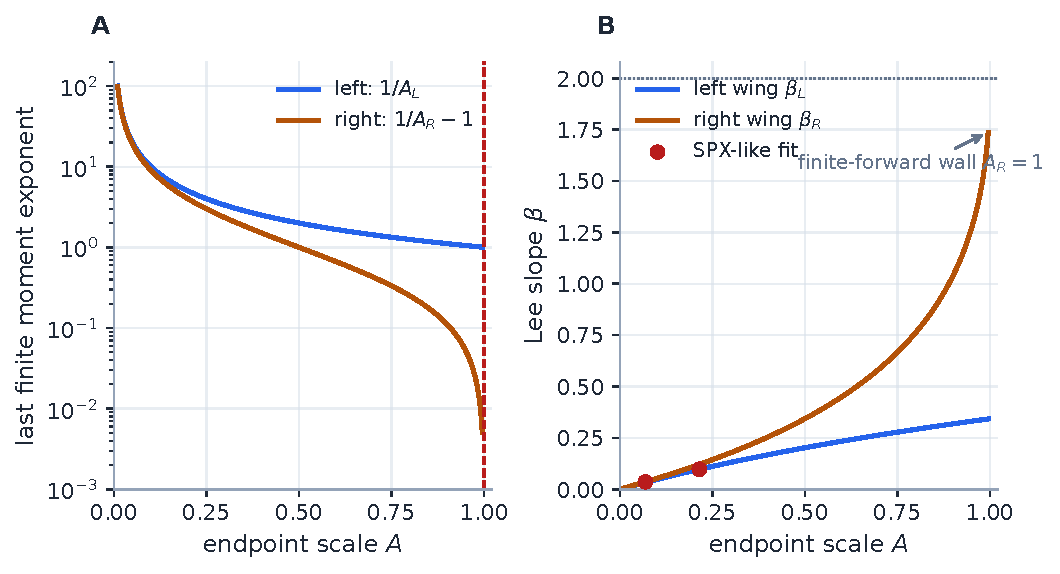
\includegraphics[width=\textwidth]{fig_lqd_tail_map.pdf}
\caption{The endpoint scales carry economic meaning.  Panel A maps each scale
to its last finite moment; the right moment collapses at $A_R=1$.  Panel B maps
the same scales to Lee slopes.  The red points are the two tails of the
SPX-like benchmark: they sit far from the wall and well below the slope ceiling.}
\label{fig:tail_map}
\end{figure}

\begin{example}[title={Example: reading the SPX-like tails}]
The fitted benchmark later studied in \cref{sec:svi_case} has
$A_L=\lqdsviAL$ and $A_R=\lqdsviAR$.  Equations
\eqref{eq:critical_moments}--\eqref{eq:lee_slopes} give
$\beta_L=\lqdsvibetaL$ and $\beta_R=\lqdsvibetaR$.  These are sensible
extrapolation diagnostics, not strongly identified market observables:
twenty-five quotes over a finite strike window cannot uniquely determine
asymptotic moments.
\end{example}

%======================================================================
\section{Pricing is one cumulative integral}
\label{sec:pricing}

The percentile formula \eqref{eq:call_u} is conceptually complete.  Production
re-expresses it on the logit grid because that grid is smooth, symmetric and
shared by every strike.

\subsection{Normalize once, then reuse the upper asset share}

Start from the centred primitive \eqref{eq:qbar}.  Since
$\dd u=u(1-u)\dd z$, the martingale shift is
\begin{equation}
\mu=-\log\!\left[
\int_{-\infty}^{\infty}
e^{\overline Q(z)}\Lambda(z)(1-\Lambda(z))\dd z
\right],
\qquad
Q(z)=\mu+\overline Q(z).
\label{eq:mu}
\end{equation}
Define the upper asset-share integral
\begin{equation}
\mathcal A(z)
=\int_z^\infty e^{Q(r)}\Lambda(r)(1-\Lambda(r))\dd r.
\label{eq:asset_share}
\end{equation}
If $z_k$ solves $Q(z_k)=k$ and $u_k=\Lambda(z_k)$, then
\begin{equation}
C(k)=\mathcal A(z_k)-e^k(1-u_k).
\label{eq:call_z}
\end{equation}
This is just \eqref{eq:call_u} split into its asset and strike legs.  One
forward cumulative integral builds $Q$; one reverse cumulative integral builds
$\mathcal A$; each strike then needs only a scalar inversion and interpolation.

\subsection{From price to the quoted Black volatility}

The normalized Black call in total-variance coordinates is
\begin{equation}
\Black(k,w)=\PhiN(d_+)-e^k\PhiN(d_-),
\qquad
d_\pm=-\frac{k}{\sqrt w}\pm\frac{\sqrt w}{2}.
\label{eq:black}
\end{equation}
For an admissible call price, implied total variance solves
$\Black(k,w(k))=C(k)$, and
\begin{equation}
\sigma_{\rm imp}(k)=\sqrt{\frac{w(k)}{\tau}}.
\end{equation}
LQD therefore does not interpolate in implied-volatility space.  The full
strike curve, including its extrapolation, is the Black image of a fitted
probability distribution.

\subsection{What the finite grid actually computes}
\label{sec:numerics}

The production grid is $z\in[-40,40]$.  Optimization uses \lqdoptpts\ nodes;
the accepted slice is rebuilt once on $8001$ nodes for reporting and downstream
diagnostics.  Cumulative Simpson integration constructs $Q$ and $\mathcal A$
when available, while the martingale body integral uses the trapezoidal rule.
At the two truncated endpoints the leading asymptotic corrections are
\begin{equation}
\int_{40}^{\infty} e^Q u(1-u)\dd z
\approx\frac{e^{Q(40)-40}}{1-A_R},
\qquad
\int_{-\infty}^{-40} e^Q u(1-u)\dd z
\approx\frac{e^{Q(-40)-40}}{1+A_L}.
\label{eq:tail_corrections}
\end{equation}
For a fixed finite-order polynomial $g$, the neglected relative terms decay
exponentially in the cutoff.  They are tiny for ordinary fitted equity scales,
but \eqref{eq:tail_corrections} remains an asymptotic correction, not an exact
tail integral.

At each grid node the implementation stores
\[
Q_z=e^g,\qquad
\mathcal A_z=-e^Q u(1-u).
\]
These exact nodal derivatives define cubic-Hermite interpolants.  Strike
inversion starts from a linear seed and takes four safeguarded Newton steps.
On benchmark slices this is much more accurate than a table lookup; it should
not be advertised as a universal extrapolator outside the finite grid or as an
algebraic proof of machine precision for arbitrary coefficients.

\begin{perfbox}
The arrays $(z,u,u(1-u))$ and the Legendre matrix depend only on grid size and
model order.  They are cached and returned read-only.  Calibration reforms only
$g$, its exponential and the cumulative integrals.  The static-grid cache made
\texttt{build\_slice} about $1.7\times$ faster; the two-grid scheme spends full
resolution only on the accepted parameters.
\end{perfbox}

%======================================================================
\section{Exact ATM handles: level, digital mismatch and density}
\label{sec:atm}

Traders rarely want to drag $a_4$ on a screen.  They want ATM volatility, ATM
skew and ATM curvature.  LQD obtains these as analytic log-strike derivatives
of the numerically constructed slice, without finite-differencing an implied-vol
grid.

Let $u_0$ solve $Q(u_0)=0$ and define
\begin{equation}
c_0=C(0),\qquad
f_0=f_X(0)=u_0(1-u_0)e^{-g(u_0)}.
\label{eq:atm_inputs}
\end{equation}
Differentiating the call expectation with respect to log strike gives
\begin{equation}
C'(0)=-(1-u_0),\qquad
C''(0)=f_0-(1-u_0).
\label{eq:call_atm_derivatives}
\end{equation}
The ATM Black identity is
\[
c_0=2\PhiN\!\left(\frac{\sqrt{w_0}}{2}\right)-1,
\]
so its solution is explicit:
\begin{equation}
w_0=4\left[
\PhiN^{-1}\!\left(\frac{1+c_0}{2}\right)
\right]^2.
\label{eq:w0}
\end{equation}
Set
\begin{equation}
d_0=\frac{\sqrt{w_0}}{2},\qquad
\varphi_0=\phin(d_0),\qquad
\delta=u_0-\PhiN(d_0).
\label{eq:atm_short}
\end{equation}
Implicit differentiation of $\Black(k,w(k))=C(k)$ and elementary simplification
give
\begin{align}
w'(0)
  &=2\sqrt{w_0}\,\frac{\delta}{\varphi_0}, \label{eq:wprime}\\
w''(0)
  &=2\sqrt{w_0}\,\frac{f_0}{\varphi_0}-2
    +2\left(1+\frac{w_0}{4}\right)
       \left(\frac{\delta}{\varphi_0}\right)^2.
\label{eq:wsecond}
\end{align}
Converting total variance to annualized volatility yields the three handles
\begin{align}
\sigma_0
  &=\sqrt{\frac{w_0}{\tau}}, \label{eq:sigma0}\\
s_0
  &=\left.\frac{\partial\sigma_{\rm imp}}{\partial k}\right|_{0}
   =\frac{\delta}{\varphi_0\sqrt{\tau}}, \label{eq:skew0}\\
\kappa_0
  &=\left.\frac{\partial^2\sigma_{\rm imp}}{\partial k^2}\right|_{0}
   =\frac{1}{\sqrt{\tau}}\left[
      \frac{f_0}{\varphi_0}-\frac{1}{\sqrt{w_0}}
      +\frac{\sqrt{w_0}}{4}
       \left(\frac{\delta}{\varphi_0}\right)^2
     \right].
\label{eq:curv0}
\end{align}

\begin{proposition}[What the ATM handles measure]
\label{prop:atm}
For any admissible numerically constructed LQD slice, the identities
\eqref{eq:sigma0}--\eqref{eq:curv0} give its exact analytic log-strike ATM
derivatives.  Level is determined by the ATM call, skew by the difference
between the LQD and Black ATM CDF levels $u_0$ and $\PhiN(d_0)$
(equivalently, the negative call-digital mismatch), and curvature primarily by
the density height $f_0$, with a skew correction.
\end{proposition}

\begin{proof}
Equation \eqref{eq:call_atm_derivatives} follows from
$C'(k)=-e^k(1-F_X(k))$.  Differentiate the identity
$\Black(k,w(k))=C(k)$ once and twice, substitute the Black partial derivatives
at $k=0$, and simplify using \eqref{eq:atm_short}.  Finally differentiate
$\sigma_{\rm imp}=\sqrt{w/\tau}$.
\end{proof}

The qualifier \emph{numerically constructed} matters.  $u_0$, $c_0$ and $f_0$
come from the quadrature slice.  The formulas are exact chain-rule identities
conditional on that slice; they are not closed-form functions of the raw
coefficient vector.

%======================================================================
\section{A local chart in trader coordinates}
\label{sec:chart}

Let $\theta=(L,R,a_2,\ldots,a_N)\in\R^d$ and collect the internal chart handles
as
\begin{equation}
H(\theta)=(w_0,s_0,\kappa_0).
\end{equation}
The graph-facing carrier used by Note~14 replaces $w_0$ with
$\sigma_0=\sqrt{w_0/\tau}$; the distinction is small in notation and important
in units.

\begin{assumption}[Regular handle point]
\label{ass:rank}
At the reference slice $\theta^*$, the Jacobian
$J=\partial H/\partial\theta\in\R^{3\times d}$ has full row rank three and is
not numerically ill-conditioned in the chosen Euclidean coefficient metric.
\end{assumption}

Under \cref{ass:rank}, let $J^\dagger=J\T(JJ\T)^{-1}$ be the least-norm right
inverse and let the columns of $V$ form an orthonormal basis of $\ker J$.  A
local displacement can be written
\begin{equation}
\theta=\theta^*+J^\dagger\alpha+V\xi.
\label{eq:chart}
\end{equation}
To first order, $\alpha\in\R^3$ moves the three trader handles one-for-one,
while the shape coordinate $\xi\in\R^{d-3}$ leaves them unchanged:
$J J^\dagger=I_3$ and $JV=0$.  In code, an SVD/QR construction is preferable
near weak rank because it exposes the small singular values rather than hiding
them in $(JJ\T)^{-1}$.

For a finite move, first-order orthogonality is not enough.  Production holds
$\xi$ fixed and solves the three-dimensional nonlinear equation
\begin{equation}
H(\theta^*+J^\dagger\alpha+V\xi)=H_{\rm target}
\label{eq:retarget}
\end{equation}
by Newton iteration.  This keeps the chart's local shape coordinates fixed; it
does \emph{not} promise that the endpoint scales or wings remain unchanged.

\begin{caution}
The chart is local and conditional on rank.  A large handle request can leave
the neighbourhood where $J$ is useful, drive $A_R$ toward the integrability
wall, or admit no feasible retargeted slice.  The chart separates tasks; it
does not regularize the free shape coordinates.  Ridge penalties, data and
priors remain responsible for suppressing implausible oscillation.
\end{caution}

%======================================================================
\section{Calibration: fit prices, measure errors in volatility units}
\label{sec:calibration}

\subsection{The core objective}

Suppose the prepared quote set contains $(k_i,\sigma_i,\omega_i)$ at active
time $\tau$, with quote total variance $w_i=\sigma_i^2\tau$.  Convert each
quote once to its normalized Black call and freeze its quote vega:
\begin{equation}
C_i^{\rm mkt}=\Black(k_i,w_i),\qquad
v_i=\phin(d_{+,i})\sqrt{\tau}.
\end{equation}
The core fit minimizes
\begin{equation}
\sum_i\omega_i
\left(
\frac{C^{\rm LQD}(k_i;\theta)-C_i^{\rm mkt}}
     {v_i+\eta}
\right)^2
+\lambda\sum_{n=4}^{N}n^{2r}a_n^2.
\label{eq:objective}
\end{equation}
The price numerator preserves the distribution-first construction at each
feasible priced iterate.  Dividing by quote vega makes the residual locally
comparable to a volatility error; the floor $\eta=10^{-4}$ prevents far-wing
quotes from receiving explosive weight.  The high-order ridge leaves
$a_2,a_3$ free and damps modes $n\ge4$.

The low-level function defaults to $\lambda=0$.  The shipped application
setting is $\lambda=10^{-6}$, and the benchmark generator passes it explicitly.
This distinction matters when reproducing a fit from the library rather than
the UI.

\subsection{The soft turn before the hard wall}

The residual stack always contains the softplus row
\begin{equation}
b(\theta)=\log\!\left(1+
\exp\{s_b(A_R-c)\}\right),
\qquad c=\lqdbarriercenter,\quad s_b=\lqdbarrierscale.
\label{eq:barrier}
\end{equation}
It is evaluated with a stable \texttt{logaddexp}.  When a trial reaches the
buffered hard wall $A_R\ge1-10^{-6}$, slice construction is skipped and the
price block is replaced by a large penalty increasing with $A_R$.  Thus an
infeasible trust-region trial does not produce a fake option surface; it
receives a direction back toward feasibility.

\subsection{Initialization and warm starts}

The cold start is the logistic family of \cref{sec:logistic}:
\begin{equation}
s_{\rm init}=\frac{\sqrt{3w_{\rm ATM}}}{\pi},\qquad
L=R=\log s_{\rm init},\qquad a_n=0.
\label{eq:cold_start}
\end{equation}
As the logistic example showed, this is a scale heuristic rather than an exact
ATM match.  In a surface sweep, the fitted shorter expiry is usually a much
better initializer for the next expiry.  The production workflow therefore
fits nearest to farthest and warm-starts sequentially.  A data-only prepass can
also supply the measurement stage for the persistence and filtering machinery
of Notes~13 and 15.

\subsection{The production residual stack}
\label{sec:residual_stack}

The core objective is only the spine.  \texttt{calibrate\_slice} concatenates
the blocks in \cref{tab:stack}.  Optional blocks are absent when inactive, and
the Jacobian route changes with them.

\begin{table}[H]
\centering\small
\setlength{\tabcolsep}{4pt}
\begin{tabular}{@{}p{0.28\textwidth}p{0.28\textwidth}p{0.22\textwidth}p{0.12\textwidth}@{}}
\toprule
Block & Activation & Scale & Jacobian\\
\midrule
Mid or band quote data & selected fit mode & vega-normalized price & analytic\\
High-order ridge & $\lambda>0$ & coefficient residual & analytic\\
Calendar hinge & nearer fitted expiry available and control on & asset share &
analytic\\
$A_R$ barrier & always & dimensionless & analytic\\
\midrule
Market var-swap & active quote and toggle & volatility & FD\\
Strike-gap prior & active prior mode & vega-normalized price & FD\\
Prior var-swap & active companion prior & volatility & FD\\
Operator/filter prior & gated prior or active filter & handle/operator units &
FD\\
\bottomrule
\end{tabular}
\caption{The production residual stack.  FD denotes scipy's two-point
finite-difference Jacobian; activating any var-swap or prior block switches the
entire solve to that route.}
\label{tab:stack}
\end{table}

%======================================================================
\section{Case file: an SPX-like smile}
\label{sec:svi_case}

The first test is deliberately synthetic.  It asks whether seven LQD
parameters can approximate a clean, familiar equity-index shape; it is not a
claim about live market fit.  At $\tau=0.5$, the target is raw SVI
\begin{equation}
w_{\rm SVI}(k)
=a+b\left\{\rho(k-m)+\sqrt{(k-m)^2+\sigma_{\rm SVI}^2}\right\},
\label{eq:svi}
\end{equation}
with
\[
(a,b,\rho,m,\sigma_{\rm SVI})
=(0.010625,\;0.07289,\;-0.5,\;0.05831,\;0.10100).
\]
Twenty-five synthetic quotes cover $k\in[-0.35,0.30]$.  The production
calibrator uses $N=6$, the application ridge $\lambda=10^{-6}$, equal quote
weights, the logistic cold start and the standard barrier.

\begin{figure}[H]
\centering
\begin{minipage}{0.49\textwidth}\centering
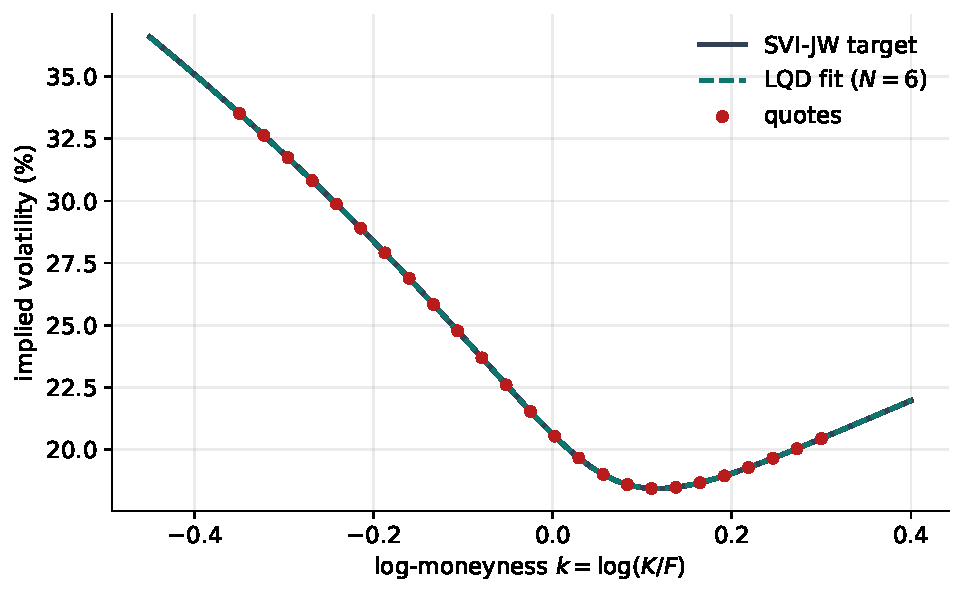
\includegraphics[width=\textwidth]{fig_lqd_svi_fit.pdf}
\end{minipage}\hfill
\begin{minipage}{0.49\textwidth}\centering
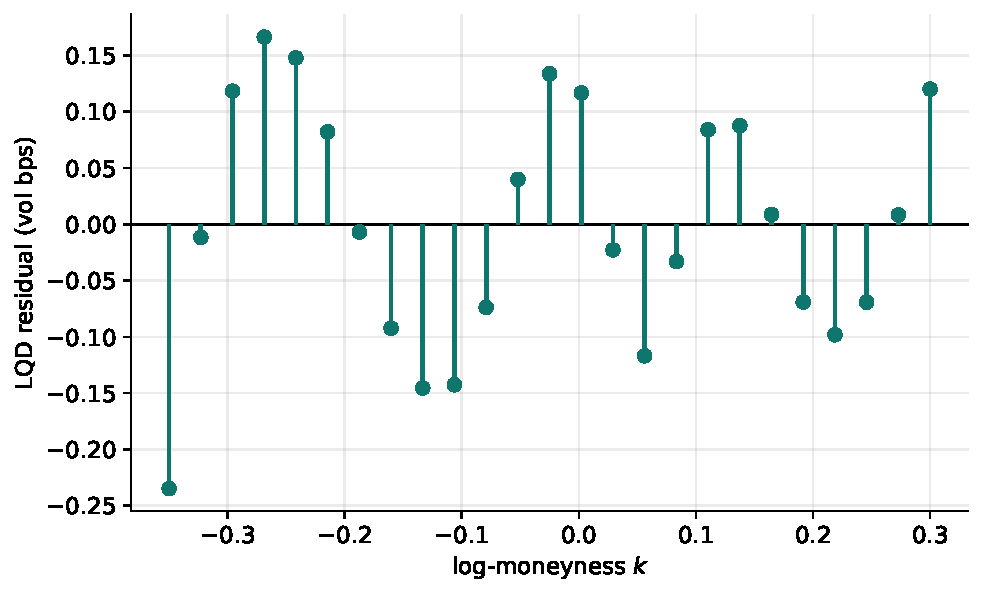
\includegraphics[width=\textwidth]{fig_lqd_svi_error.pdf}
\end{minipage}
\caption{The seven-parameter LQD slice is visually indistinguishable from the
SVI target over the quote window (left), but the residual panel (right) makes
the approximation claim auditable: the maximum quote-grid error is
\lqdsvimaxerr\ volatility basis points.  Outside the fitted window the LQD
curve follows its own distributional tails, not an SVI continuation.}
\label{fig:svi_fit}
\end{figure}

The fit takes \lqdsvinfev\ residual evaluations.  Its exact ATM readout is
\[
\sigma_0=\lqdsvisigma\%,\qquad
s_0=\lqdsviskew,\qquad
\kappa_0=\lqdsvicurv.
\]
The martingale self-consistency check is
$\E[e^X]-1=\lqdsvimart$.  The endpoint and tail diagnostics are
\[
A_L=\lqdsviAL,\quad A_R=\lqdsviAR,\quad
\beta_L=\lqdsvibetaL,\quad \beta_R=\lqdsvibetaR.
\]
Raw SVI has asymptotic slopes $b(1-\rho)=0.1093$ on the left and
$b(1+\rho)=0.0364$ on the right.  Their closeness to the LQD diagnostics is
reassuring for this constructed target, but finite-window quotes do not in
general identify asymptotic slopes to two decimals.

\begin{figure}[H]
\centering
\begin{minipage}{0.49\textwidth}\centering
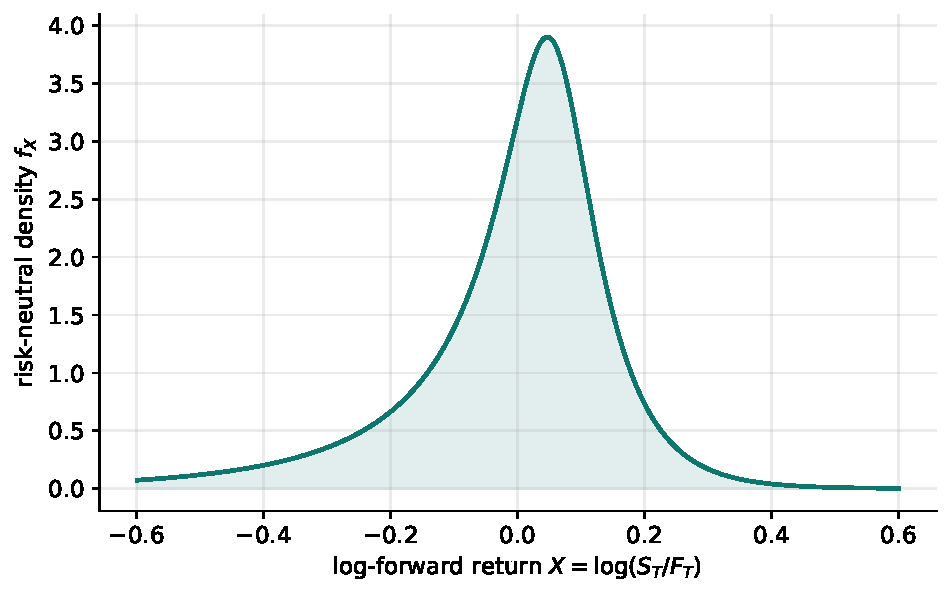
\includegraphics[width=\textwidth]{fig_lqd_density.pdf}
\end{minipage}\hfill
\begin{minipage}{0.49\textwidth}\centering
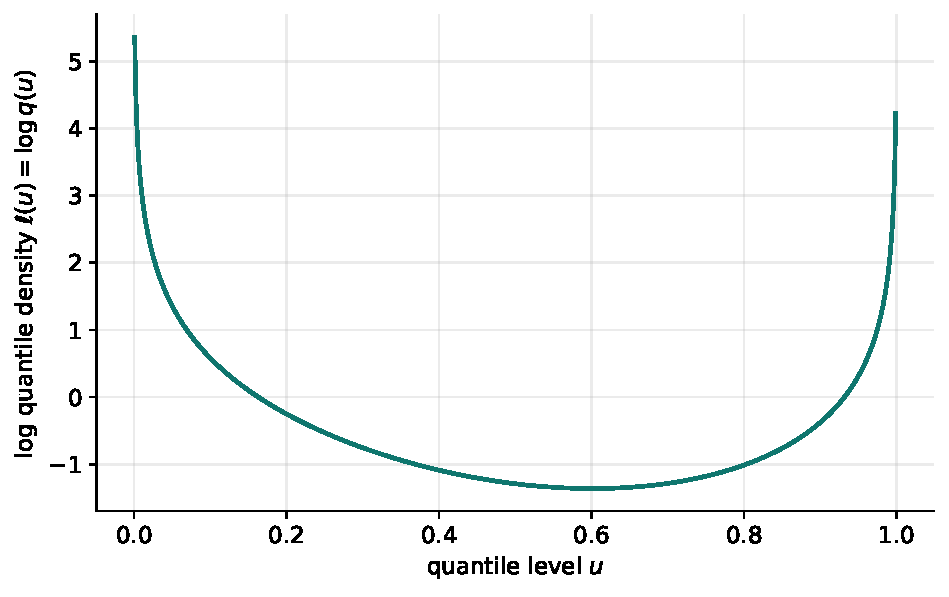
\includegraphics[width=\textwidth]{fig_lqd_logq.pdf}
\end{minipage}
\caption{The same fit in distribution coordinates.  The log-return density is
non-negative because it is the reciprocal of a positive quantile density
(left).  The log quantile density (right) shows the endpoint rise that produces
exponential return tails.  Positivity is structural; the economic plausibility
of the shape still comes from data and regularization.}
\label{fig:svi_distribution}
\end{figure}

\begin{table}[H]
\centering
\caption{Fresh seven-parameter LQD fit to the SPX-like SVI target.  Because the
basis is global, the coefficients should not be read individually as pure
level, skew, curvature or wing knobs.}
\label{tab:svi_coefficients}
\lqdsvicoefftable
\end{table}

\begin{example}[title={Case verdict: approximation capacity, not market alpha}]
\textbf{Setup:} a clean six-month index-like SVI smile.
\textbf{Failure to avoid:} matching the quotes while creating negative density
between them.
\textbf{Mechanism:} fit normalized prices inside the LQD density family.
\textbf{Verdict:} \lqdsvimaxerr\ vol bp maximum error on the twenty-five input
quotes, a non-negative density and a finite-forward tail far from the wall.
Live bid--ask and out-of-sample comparisons belong to
\texttt{backend/backtest/}, not to this synthetic case.
\end{example}

%======================================================================
\section{Case file: the density wears two hats}
\label{sec:doublehat}

Scheduled elections, court decisions, earnings and binary regulatory events can
produce a terminal law with two plausible landing zones.  To isolate that
geometry, take the equal mixture
\begin{equation}
X\sim\frac12N(m_1,s^2)+\frac12N(m_2,s^2),
\qquad
(m_1,m_2,s)=(-0.10075573,\;0.08924427,\;0.05).
\label{eq:mixture}
\end{equation}
Here $s=5\%$ is the component standard deviation of the thirty-day
\emph{log-return}, not an annualized implied volatility.  The means are chosen
so
\begin{equation}
\frac12e^{m_1+s^2/2}+\frac12e^{m_2+s^2/2}=1,
\end{equation}
which martingale-normalizes the mixture.  Its call is available in closed form:
\begin{equation}
C_{\rm mix}(k)
=\frac12\sum_{j=1}^{2}\left[
e^{m_j+s^2/2}
\PhiN\!\left(\frac{m_j+s^2-k}{s}\right)
-e^k\PhiN\!\left(\frac{m_j-k}{s}\right)
\right].
\label{eq:mixture_call}
\end{equation}
We turn forty-one such calls over $k\in[-0.25,0.25]$ into implied variances and
fit $N=12$ with $\lambda=10^{-7}$.

\begin{figure}[H]
\centering
\begin{minipage}{0.49\textwidth}\centering
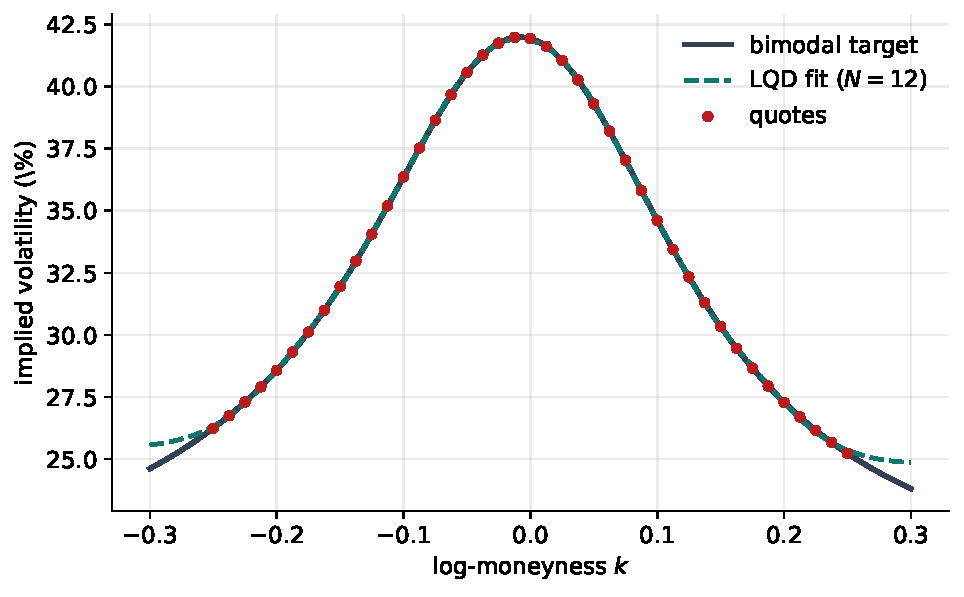
\includegraphics[width=\textwidth]{fig_lqd_doublehat.pdf}
\end{minipage}\hfill
\begin{minipage}{0.49\textwidth}\centering
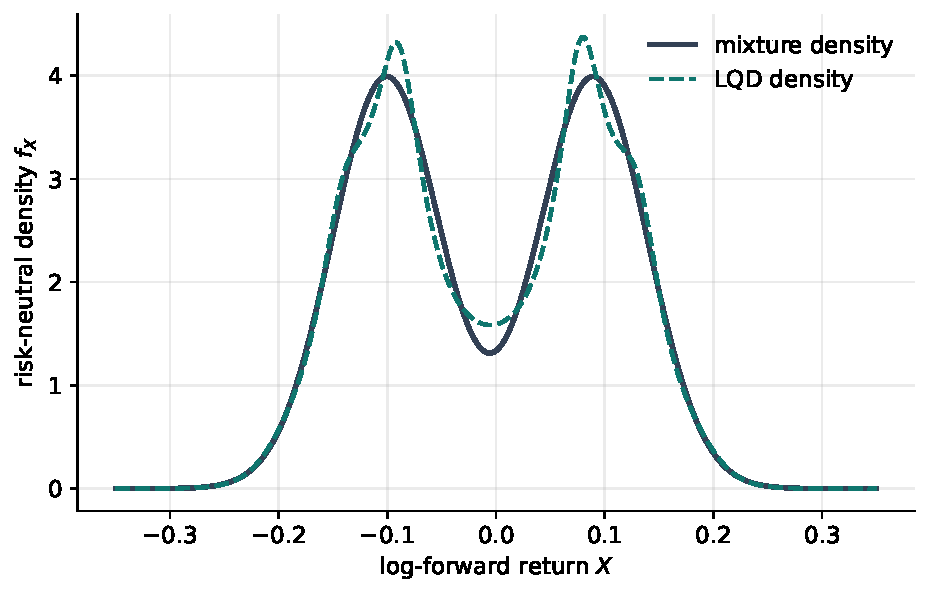
\includegraphics[width=\textwidth]{fig_lqd_doublehat_dens.pdf}
\end{minipage}
\caption{A binary-event geometry needs more than a smooth U-shaped smile.
The thirteen-parameter fit captures the central trough and supported wings
(left) and qualitatively recovers both modes of the known target density
(right).  The maximum quote-grid error is \lqddhmaxerr\ vol bp; the density
comparison is possible only because this is a synthetic case with a known law.}
\label{fig:doublehat}
\end{figure}

The fitted endpoint scales are $A_L=\lqddhAL$ and $A_R=\lqddhAR$, both thin and
far from the integrability wall.  Higher order is doing real work in the
centre, but positivity alone does not certify that the two modes are genuine.
With sparse quotes, a high-order LQD slice can create a beautifully admissible
fiction.

\begin{example}[title={Case verdict: positive is not the same as plausible}]
\textbf{Setup:} a known two-normal event mixture.
\textbf{Failure to avoid:} forcing a low-order smile through a central trough,
or using an unconstrained flexible curve that turns negative between quotes.
\textbf{Mechanism:} higher Legendre order inside an always-positive quantile
density.
\textbf{Verdict:} both modes are qualitatively recovered, with
\lqddhmaxerr\ vol bp maximum quote-grid error.  On real data, order selection,
ridge strength, bid--ask information and event priors must decide whether a
second hat is signal or overfit.
\end{example}

%======================================================================
\section{The free derivative: an envelope argument}
\label{sec:jacobian}

For a seven-parameter fit, a finite-difference Jacobian rebuilds the quadrature
once for the value and once per bumped coefficient.  That is tolerable; at
higher order and across many expiries it becomes the dominant repeated work.
The continuous price formula contains a fortunate cancellation.

Let $u_k(\theta)$ be the moving percentile satisfying
$Q(u_k(\theta);\theta)=k$.  Differentiate \eqref{eq:call_u} at fixed strike:
\begin{align}
\frac{\partial C(k;\theta)}{\partial\theta}
&=\int_{u_k}^{1}
e^{Q(u;\theta)}Q_\theta(u;\theta)\dd u
-\left[e^{Q(u_k;\theta)}-e^k\right]
\frac{\partial u_k}{\partial\theta} \nonumber\\
&=\int_{u_k}^{1}
e^{Q(u;\theta)}Q_\theta(u;\theta)\dd u.
\label{eq:envelope}
\end{align}
The boundary term vanishes because $Q(u_k;\theta)=k$.  The strike root may move
violently with a parameter; its first-order effect on the payoff is still zero
because the payoff itself is zero at the exercise boundary.

\begin{theorem}[Implicit-root cancellation]
\label{thm:envelope}
For an admissible smooth LQD slice, the parameter derivative of a fixed-strike
call is the explicit quantile sensitivity in \eqref{eq:envelope}.  No derivative
of the implicit strike root is required.
\end{theorem}

\begin{proof}
Apply Leibniz' rule to \eqref{eq:call_u}.  The moving-boundary term is the payoff
at the boundary times $u_{k,\theta}$, and the payoff is zero.
\end{proof}

In logit coordinates, production evaluates the same derivative by interpolating
the parameter sensitivities of the upper asset share at the fixed $z_k$.  If
$\phi_j(u)=\partial g/\partial\theta_j$, then
\begin{equation}
\frac{\partial\overline Q(z)}{\partial\theta_j}
=\int_0^z e^{g(\Lambda(r))}\phi_j(\Lambda(r))\dd r,
\label{eq:q_sensitivity}
\end{equation}
where
\[
\phi_L=1-u,\qquad \phi_R=u,\qquad
\phi_{a_n}=P_n(1-2u).
\]
Differentiate the martingale normalization, add the resulting scalar
$\mu_{\theta_j}$ to \eqref{eq:q_sensitivity}, and reverse-integrate
$e^Qu(1-u)Q_{\theta_j}$ to obtain the asset-share sensitivity.  The endpoint
corrections also differentiate through $Q(\pm40)$ and $A_L,A_R$.  Ridge,
calendar and barrier rows then add elementary derivatives.

The theorem is exact for the continuous integrals.  The production price and
gradient use separately constructed Hermite interpolants, so an off-node
comparison inherits a small discretization mismatch.  The tested claim is
numerical: on mid, band and calendar residual stacks the analytic Jacobian
agrees with a three-point finite difference to relative tolerance $10^{-3}$,
and analytic and two-point-FD fits reach coefficient vectors within about
$10^{-5}$ and costs agreeing near $10^{-11}$ relative.

\begin{figure}[H]
\centering
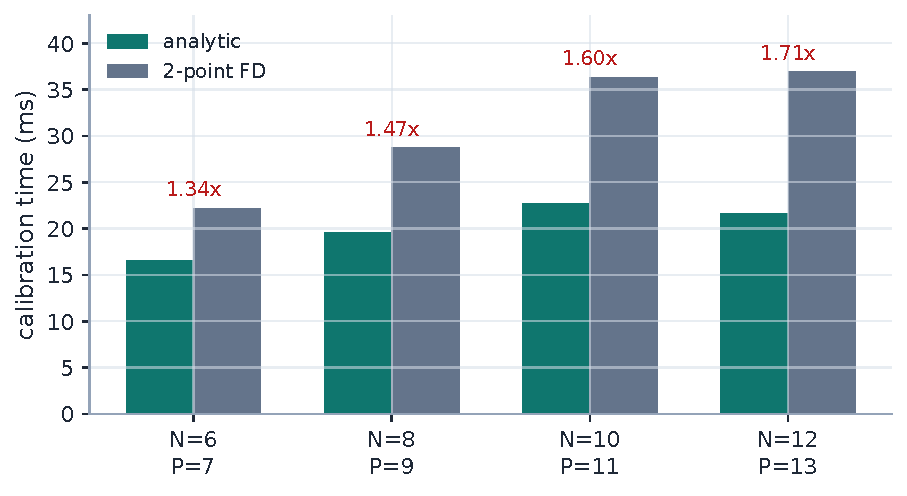
\includegraphics[width=0.88\textwidth]{fig_lqd_jacobian_timing.pdf}
\caption{The envelope cancellation removes repeated quadrature builds.  On the
warm-cache optimizer-core benchmark, the analytic route is
$1.34$--$1.71\times$ faster over $N=6,\ldots,12$ and reaches the same optimum
within the tested tolerances.  These bars exclude the final full-grid rebuild
and reporting work, so they are not end-to-end API latency.}
\label{fig:jacobian_timing}
\end{figure}

\begin{heuristic}
Why is the speed-up not $P$-fold for $P$ parameters?  Cached static arrays make
each bumped build relatively cheap, the trust-region solve still performs
linear algebra and value evaluations, and these clean synthetic fits converge
in few iterations.  The useful result is structural: higher order no longer
forces one full quadrature rebuild per Jacobian column.
\end{heuristic}

%======================================================================
\section{From slices to a surface: convex order, softly enforced}
\label{sec:calendar}

Butterfly freedom is a within-expiry property.  For expiry dates
$T_1<T_2$, absence of calendar arbitrage under deterministic carry requires
\begin{equation}
C_{T_1}(k)\le C_{T_2}(k)\qquad\text{for every }k.
\label{eq:calendar_calls}
\end{equation}
Because both normalized underlyings have mean one, this is equivalent to saying
that $Y_{T_2}$ dominates $Y_{T_1}$ in convex order: the later law is more
dispersed without moving its mean.

Quantiles give a native criterion.  Define the integrated upper quantile
\begin{equation}
G_T(\alpha)=\int_\alpha^1e^{Q_T(u)}\dd u,
\qquad 0\le\alpha\le1.
\label{eq:upper_quantile}
\end{equation}
For equal-mean positive laws,
\begin{equation}
Y_{T_1}\le_{cx}Y_{T_2}
\quad\Longleftrightarrow\quad
G_{T_1}(\alpha)\le G_{T_2}(\alpha)
\quad\text{for every }\alpha,
\label{eq:convex_order}
\end{equation}
with equality at $\alpha=0$.  In LQD, $G_T(\Lambda(z))$ is exactly the asset
share $\mathcal A_T(z)$ already present on the pricing grid.

Production fits nearest to farthest.  When calendar control is on, a new slice
receives hinge residuals whenever its asset share falls below the previous
slice at sampled logit nodes.  The comparison is expressed at $z$ values, so
the same locations can be evaluated on either the optimization or reporting
grid.

\begin{caution}
The mathematical condition \eqref{eq:convex_order} is a continuum condition.
Production samples it, assigns a finite penalty weight, and allows the control
to be switched off.  It is therefore calendar \emph{control}, not a hard
guarantee.  A later independent single-expiry refit has no neighbouring-slice
context and can also break a previously coupled surface.  Diagnostics must
measure the final call ordering rather than infer it from the workflow.
\end{caution}

Note~10 treats the model-agnostic calendar problem in detail.  LQD's advantage
is not a stronger theorem; it is that the natural convex-order object is already
one of its cumulative pricing arrays.

%======================================================================
\section{The native log-contract route}
\label{sec:varswap}

For a mean-one positive underlying, the continuous log-contract proxy to total
variance is
\begin{equation}
w_{\rm vs}=-2\E[X]
=-2\int_0^1Q(u)\dd u
=-2\int_{-\infty}^{\infty}
Q(z)\Lambda(z)(1-\Lambda(z))\dd z.
\label{eq:varswap}
\end{equation}
The last integral uses the grid LQD already owns.  Production evaluates it by
a trapezoidal rule without explicit tail corrections; its integrand decays as
$z e^{-|z|}$, so the omitted $|z|>40$ contribution is negligible in ordinary
double precision.

Equation \eqref{eq:varswap} prices a log contract.  Identifying it with a
realized-variance swap assumes the usual continuous-monitoring, continuous-path
convention.  Jumps and discrete sampling require corrections.  Activating the
market var-swap residual also switches the whole calibration to the
finite-difference Jacobian because this optional block has not yet been added
to the analytic route.

%======================================================================
\section{What is guaranteed, and what is merely hoped for}
\label{sec:limits}

\Cref{tab:contract} is the shortest honest description of the model.

\begin{table}[H]
\centering\small
\setlength{\tabcolsep}{5pt}
\begin{tabular}{@{}p{0.30\textwidth}p{0.29\textwidth}p{0.33\textwidth}@{}}
\toprule
Property & Status & Qualification\\
\midrule
Non-negative continuous density & Structural & For every finite coefficient
vector; numerical pricing is still finite precision.\\
One-expiry butterfly freedom & Structural after normalization & Requires a
finite forward and correct normalized units.\\
Finite forward & If and only if $A_R<1$ mathematically & Code uses the buffer
$A_R<1-10^{-6}$.\\
Exponential $X$ tails and Lee-consistent wings & Structural & A modelling
choice; finite strikes weakly identify the scales.\\
ATM level, skew and curvature & Analytic slice identities & Conditional on the
numerically built slice; not raw-coefficient closed forms.\\
\midrule
Calendar freedom & Not structural & Sampled, finite-weight, optional control.\\
Economically plausible density & Not guaranteed & High order can fit noise or
invent modes while remaining positive.\\
Atoms at zero or elsewhere & Not represented & The law is continuous; sharp
continuous features only approximate mass points.\\
Unique or stable coefficients & Not guaranteed & Sparse quotes create nearly
flat parameter directions; compare prices, handles and densities instead.\\
Market superiority & Not established here & The cases are deterministic
synthetic approximation tests.\\
\bottomrule
\end{tabular}
\caption{The LQD contract.  Arbitrage structure and economic plausibility are
different promises.}
\label{tab:contract}
\end{table}

Three further limitations matter in practice.
\begin{itemize}[leftmargin=1.4em]
\item \textbf{Near-wall conditioning.}  As $A_R\uparrow1$, the martingale tail
correction and its derivatives dominate.  A technically feasible slice close
to the wall is fragile, and the orthogonal retarget can fail.
\item \textbf{Global modes.}  A local-looking smile improvement can alter both
endpoint scales because every Legendre polynomial reaches the endpoints.
Fitted coefficient vectors are therefore poor objects for cross-date comparison.
\item \textbf{Density inference.}  Option prices smooth the density twice.
Even a sub-vol-bp fit does not identify narrow density features; digitals,
one-touches and event probabilities deserve separate stability tests.
\end{itemize}

%======================================================================
\section{What the implementation exploits}
\label{sec:contributions}

Quantile models, density-first option pricing, Legendre expansions and Lee's
moment formula are classical ingredients.  The useful contribution is their
combination into a production coordinate system:
\begin{enumerate}[leftmargin=1.6em]
\item The endpoint skeleton in \eqref{eq:lqd} turns positivity and two-sided
tail regularity into a short unconstrained expansion, with only the genuine
right-moment wall left hard.
\item The ATM identities in \cref{sec:atm} translate the distribution into
actual trader handles, while the local null-space chart separates handle moves
from remaining first-order shape directions.
\item The envelope cancellation in \cref{thm:envelope} lets the price Jacobian
reuse the same cumulative integrals as pricing rather than differentiating an
implicit strike root or rebuilding the slice per parameter.
\end{enumerate}
None of these statements requires claiming that a generic calculus identity is
new.  The engineering value lies in choosing coordinates that make the
identities cheap, testable and composable with the rest of the surface system.

%======================================================================
\section{Traceability}
\label{sec:traceability}

The figures and displayed numbers are deterministic outputs of
\texttt{Docs/notes/figures/gen\_lqd.py} and
\texttt{Docs/notes/figures/gen\_lqd\_lecture.py}; LaTeX does not regenerate
them automatically.  Fresh generator values are the evidence used in this
lecture.  Some legacy benchmark fixtures intentionally retain older frozen
coefficients as regression tripwires, so raw coefficients in those fixtures
need not equal the current table.

\begingroup
\small
\setlength{\tabcolsep}{4pt}
\renewcommand{\arraystretch}{1.15}
\begin{longtable}{@{}p{0.29\textwidth}p{0.15\textwidth}p{0.52\textwidth}@{}}
\caption{Claims, production modules and tests.}\label{tab:traceability}\\
\toprule
Claim & Mathematical anchor & Code and test anchors\\
\midrule
\endfirsthead
\toprule
Claim & Mathematical anchor & Code and test anchors\\
\midrule
\endhead
Positive density, parity, monotone and convex benchmark calls &
\cref{prop:butterfly} &
\nolinkurl{backend/volfit/models/lqd/quadrature.py}\newline
\nolinkurl{backend/tests/test_lqd_pricing.py}\\
\addlinespace
Legendre basis, endpoint scales and Lee maps &
\eqref{eq:g}, \eqref{eq:AL}--\eqref{eq:direct_lee} &
\nolinkurl{backend/volfit/models/lqd/basis.py}\newline
\nolinkurl{backend/tests/test_lqd_basis.py}\\
\addlinespace
Logit quadrature, tail corrections and Hermite pricing &
\eqref{eq:qz}, \eqref{eq:mu}--\eqref{eq:tail_corrections} &
\nolinkurl{backend/volfit/models/lqd/quadrature.py}\newline
\nolinkurl{backend/volfit/models/lqd/interp.py}\newline
\nolinkurl{backend/tests/test_lqd_pricing.py}\\
\addlinespace
ATM level, skew and curvature &
\eqref{eq:sigma0}--\eqref{eq:curv0} &
\nolinkurl{backend/volfit/models/lqd/atm.py}\newline
\nolinkurl{backend/tests/test_lqd_atm.py}\\
\addlinespace
Local orthogonal chart and exact retarget &
\eqref{eq:chart}--\eqref{eq:retarget} &
\nolinkurl{backend/volfit/models/lqd/ortho.py}\newline
\nolinkurl{backend/tests/test_lqd_ortho.py}\\
\addlinespace
Core objective, barrier, residual ordering and final rebuild &
\eqref{eq:objective}--\eqref{eq:barrier} &
\nolinkurl{backend/volfit/models/lqd/calibrate.py}\newline
\nolinkurl{backend/tests/test_lqd_calibrate.py}\\
\addlinespace
Analytic Jacobian and fit agreement &
\cref{thm:envelope} &
\nolinkurl{backend/volfit/models/lqd/jacobian.py}\newline
\nolinkurl{backend/tests/test_lqd_jacobian.py}\\
\addlinespace
Soft nearest-to-farthest calendar control &
\eqref{eq:convex_order} &
\nolinkurl{backend/volfit/calib/calendar.py}\newline
\nolinkurl{backend/volfit/calib/surface.py}\\
\addlinespace
Active-time annualization and normalized quote preparation &
\eqref{eq:variables}--\eqref{eq:call_expectation} &
\nolinkurl{backend/volfit/api/quotes.py}\newline
\nolinkurl{backend/volfit/api/service.py}\\
\addlinespace
Fresh SVI and double-hat approximation cases &
\cref{sec:svi_case,sec:doublehat} &
\nolinkurl{Docs/notes/figures/gen_lqd.py}\newline
\nolinkurl{Docs/notes/figures/lqd_numbers.json}\newline
\nolinkurl{backend/tests/benchmarks.py}\\
\bottomrule
\end{longtable}
\endgroup

\appendix
%======================================================================
\section{Hyperparameter atlas}
\label{app:atlas}

\Cref{tab:atlas} lists the controls native to LQD.  Shared quote, band,
calendar, var-swap, prior and filtering controls are derived in Notes~07, 08,
10, 13 and 15 and indexed in Note~00 rather than duplicated here.  Application
defaults are distinguished from low-level function defaults where they differ.

\begin{longtable}{p{0.25\textwidth}p{0.14\textwidth}p{0.53\textwidth}}
\caption{LQD-native controls and constants.}\label{tab:atlas}\\
\toprule
Knob & Default & Role\\
\midrule
\endfirsthead
\toprule
Knob & Default & Role\\
\midrule
\endhead
\multicolumn{3}{l}{\emph{Surfaced in FitSettings}}\\
\midrule
\texttt{nOrder} $N$ & $6$ & Highest Legendre degree; $N+1$ parameters.
Schema range $4\le N\le16$.\\
\texttt{regLambda} $\lambda$ & $10^{-6}$ & Application default for the
high-order ridge.  The direct \texttt{calibrate\_slice} function defaults to
zero.\\
\texttt{regPower} $r$ & $1.0$ & Ridge power in
$\lambda n^{2r}a_n^2$ for $n\ge4$.\\
\texttt{barrierCenter} $c$ & \lqdbarriercenter & Centre of the $A_R$ softplus
barrier; it turns the fit before the hard wall.\\
\texttt{barrierScale} $s_b$ & \lqdbarrierscale & Barrier steepness.\\
\texttt{weightScheme} & \texttt{equal} & Quote weights; the alternative
\texttt{tv\_density} scheme is described in Note~07.\\
\midrule
\multicolumn{3}{l}{\emph{Hidden numerical constants}}\\
\midrule
\texttt{Z\_MAX} & $40.0$ & Half-width of the LQD \emph{logit integration}
grid.  This is unrelated to the separate quote screen at four ATM standard
deviations.\\
\texttt{N\_POINTS} & $8001$ & Full reporting and diagnostic grid; odd so
$z=0$ is a node.\\
\texttt{OPT\_N\_POINTS} & \lqdoptpts & Coarse grid used during optimization;
accepted parameters are rebuilt at $8001$.\\
\texttt{EPS\_AR} & $10^{-6}$ & Buffer in the code bound
$A_R<1-\texttt{EPS\_AR}$.\\
\texttt{\_VEGA\_FLOOR} $\eta$ & $10^{-4}$ & Floor in vega-normalized quote
residuals.\\
Hermite--Newton steps & $4$ & Fixed safeguarded iterations after the linear
strike-inversion seed.\\
\texttt{xtol/ftol/gtol} & $10^{-10}$ & Trust-region termination tolerances.\\
\texttt{max\_nfev} & $4000$ & Residual-evaluation cap.\\
\bottomrule
\end{longtable}

%======================================================================
\section{Performance and numerical notes}
\label{app:performance}

\begin{enumerate}[leftmargin=1.6em]
\item \textbf{Cache parameter-independent arrays.}
The static logit grid, logistic factors and Legendre matrix are keyed by grid
size and order.  This removed roughly $40\%$ of a repeated slice build and made
the benchmark build about $1.7\times$ faster.
\item \textbf{Optimize coarse, report fine.}
The \lqdoptpts-node grid is already accurate well below the quote-fit budget for
the supplied cases.  Only the accepted parameters pay for the $8001$-node
rebuild.  This is an empirical error budget, not a theorem for every wild
coefficient vector.
\item \textbf{Store derivatives with values.}
Exact nodal $Q_z$ and $\mathcal A_z$ provide cubic-Hermite pricing, smoother
off-grid Greeks and the interpolation data reused by the analytic Jacobian.
\item \textbf{Differentiate the cumulative objects.}
\Cref{thm:envelope} eliminates the strike-root derivative.  The measured
$1.34$--$1.71\times$ optimizer-core speed-up in \cref{fig:jacobian_timing}
compares warm cached runs with only analytic-supported residual blocks active.
\item \textbf{Stop below economic resolution.}
Trust-region tolerances of $10^{-10}$ avoid iterations spent chasing numerical
changes far below a volatility basis point.  Tightening them to $10^{-15}$ did
not change the displayed surface in the benchmark.
\end{enumerate}

\subsection{Numerical qualifications}

\begin{itemize}[leftmargin=1.4em]
\item The Black inversion accepts prices inside strict static bounds and
brackets total variance over a finite interval.  A failure returns a non-finite
diagnostic rather than an arbitrage-free volatility by fiat.
\item \texttt{martingale\_check} repeats the same trapezoid-plus-tail
approximation used to compute $\mu$.  It is a valuable regression
self-consistency check, not an independent truncation validation.
\item Stable \texttt{logaddexp} protects the softplus itself, but forming
$A_R=\exp(g(1))$ can overflow for an astronomically large trial vector.  The
production input pipeline and trust region keep ordinary fits far from that
regime.
\item The low-level calibration core assumes sorted aligned strikes, positive
times and variances, non-negative weights and a feasible initializer.  Quote
preparation enforces those conditions before the core is called.
\end{itemize}

\subsection{SVI-JW provenance of the first case}
\label{app:svijw}

The raw-SVI tuple in \cref{sec:svi_case} is the image, at $\tau=0.5$, of the
SVI-JW tuple
\[
(v,\psi,p,c,\widetilde v)=(0.0425,\,-0.25,\,0.75,\,0.25,\,0.034).
\]
For completeness, with $w_0=v\tau$,
\begin{equation}
b=\frac{\sqrt{w_0}}{2}(p+c),\qquad
\rho=\frac{c-p}{c+p},\qquad
\chi=\rho-\frac{4\psi}{p+c}.
\end{equation}
When $p+c>0$, $|\chi|<1$ and the denominator below is nonzero,
\begin{align}
\sigma_{\rm SVI}
&=\frac{w_0-\widetilde v\tau}
{b\left((1-\rho\chi)/\sqrt{1-\chi^2}-\sqrt{1-\rho^2}\right)},\\
m&=\frac{\chi\sigma_{\rm SVI}}{\sqrt{1-\chi^2}},\qquad
a=\widetilde v\tau-b\sigma_{\rm SVI}\sqrt{1-\rho^2}.
\end{align}
This conversion only defines the synthetic target; no SVI property is used by
the LQD construction.

%======================================================================
\section{Reference implementation}
\label{app:reference}

The following NumPy/SciPy reference keeps the mathematics visible.  On the
fresh $N=6$ benchmark it reproduces the production quantile, asset share and
martingale shift to approximately $10^{-8}$ on the dense grid; its linear
off-grid interpolation is intentionally simpler than production's Hermite
interpolation.

\begin{lstlisting}[caption={A compact LQD slice and call pricer.},
label={lst:reference}]
import numpy as np
from scipy.integrate import cumulative_simpson
from scipy.special import expit

def legendre(nmax, x):
    P = np.empty((nmax + 1, x.size))
    P[0] = 1.0
    P[1] = x
    for n in range(1, nmax):
        P[n + 1] = ((2*n + 1)*x*P[n] - n*P[n - 1]) / (n + 1)
    return P

def build(theta, z):
    L, R, a = theta[0], theta[1], theta[2:]
    u = expit(z)
    P = legendre(len(a) + 1, 1 - 2*u)
    g = (1-u)*L + u*R + a @ P[2:]
    A_L = np.exp(L + a.sum())
    signs = (-1.0) ** np.arange(2, len(a) + 2)
    A_R = np.exp(R + signs @ a)
    if A_R >= 1:
        raise ValueError("infinite forward")

    dz, Z = z[1] - z[0], z[-1]
    Qbar = cumulative_simpson(np.exp(g), dx=dz, initial=0.0)
    Qbar -= Qbar[len(z)//2]
    mass = np.exp(Qbar) * u * (1-u)
    total = (np.trapezoid(mass, z)
             + np.exp(Qbar[-1]-Z)/(1-A_R)
             + np.exp(Qbar[0]-Z)/(1+A_L))
    mu = -np.log(total)
    Q = Qbar + mu

    asset_mass = np.exp(Q) * u * (1-u)
    A = cumulative_simpson(
        asset_mass[::-1], dx=dz, initial=0.0
    )[::-1]
    A += np.exp(Q[-1]-Z)/(1-A_R)
    return u, Q, A, mu

def call(k, z, u, Q, A):
    zk = np.interp(k, Q, z)
    return np.interp(zk, z, A) - np.exp(k)*(1-expit(zk))
\end{lstlisting}

\begin{thebibliography}{9}
\bibitem{BreedenLitzenberger1978}
D.~Breeden and R.~Litzenberger.
Prices of state-contingent claims implicit in option prices.
\emph{Journal of Business}, 51(4):621--651, 1978.

\bibitem{Lee2004}
R.~W.~Lee.
The moment formula for implied volatility at extreme strikes.
\emph{Mathematical Finance}, 14(3):469--480, 2004.

\bibitem{Gatheral2006}
J.~Gatheral.
\emph{The Volatility Surface: A Practitioner's Guide}.
Wiley, 2006.

\bibitem{GatheralJacquier2014}
J.~Gatheral and A.~Jacquier.
Arbitrage-free SVI volatility surfaces.
\emph{Quantitative Finance}, 14(1):59--71, 2014.

\bibitem{Strassen1965}
V.~Strassen.
The existence of probability measures with given marginals.
\emph{Annals of Mathematical Statistics}, 36(2):423--439, 1965.

\bibitem{CarrMadan1998}
P.~Carr and D.~Madan.
Towards a theory of volatility trading.
In \emph{Volatility}, Risk Books, 1998.
\end{thebibliography}

\end{document}
